\chapter{Methodology}
\label{ch:method}

\section{A common retrieval problem}
Let $q$ be a question about paper $d$, and let $\mathcal{C}_g(d)$ contain
the chunks of $d$ at granularity $g$. Fixed-size retrieval returns
\begin{equation}
R_g(q)=\operatorname{TopK}_{c\in\mathcal{C}_g(d)}s(q,c),
\qquad K=5.
\end{equation}
A question-level router replaces the fixed $g$ with a predicted
$\hat g(q)$. Its result is still one of the five available fixed-size
actions. A local router instead selects sizes for separate regions
before assembling the returned chunks.

The source paper, embedding model, candidate sizes, and metric remain
fixed within the primary comparisons. Gold evidence can create
training labels and score saved predictions, but it is not an input
to a deployed routing decision. Table~\ref{tab:methodfamilies} makes
this boundary explicit.

\begin{table}[tbp]
\centering\small
\caption{Inputs and decision units across method families. Gold evidence
is used offline for supervision or evaluation, never as a prediction input.}
\label{tab:methodfamilies}
\begin{tabularx}{\textwidth}{@{}p{3.1cm}XX@{}}
\toprule
Family & Prediction-time information & Decision\\
\midrule
Fixed size & Question embedding, source paper & Rank chunks at one preset size\\
Embedding router & Question embedding & One size per question\\
Qwen router & Question text & One size per question\\
Similarity-tree router & Question-to-chunk score structure & One size per question\\
Fusion / regret & Qwen features and similarity structure & One size per question\\
Local router & Tree-local score features & One size per selected tree\\
Local router + Qwen & Local features and a frozen question category & One size per selected tree\\
\bottomrule
\end{tabularx}
\end{table}

\section{Fixed and mixed-granularity baselines}
\subsection{Fixed-size retrieval}
The five fixed baselines differ only in the size filter. Their outputs
establish the utilities $U(q,g)$ and the oracle in
Equation~\ref{eq:oracle}. Fixed 40 is the strongest of these settings
on the preserved validation data and is used as the main operational
reference in the later comparisons. Since that designation follows
observed development results, it is not an independently selected
test-time constant.

\subsection{Pooling all levels}
Raw mixed retrieval removes the size filter and ranks candidates from
all levels together. It does not ask a classifier to choose a size.
In principle this can return both precise and contextual passages for
the same question. In practice it assumes that similarity scores are
sufficiently comparable across levels and that overlapping candidates
will not consume too much of the top-five result.

The deduplicated variant adds an overlap rule. Candidates are visited
in ranked order and a candidate is rejected when its source overlap
with an accepted chunk is too large:
\begin{equation}
\operatorname{ov}(c_i,c_j)=
\frac{|I_i\cap I_j|}{\min(|I_i|,|I_j|)}\geq 0.8,
\label{eq:overlap}
\end{equation}
where $I_i$ and $I_j$ are valid character intervals in the same paper.
The shorter-span denominator means that a small chunk nested in a
larger one can be treated as redundant even if the larger span extends
well beyond it.

The default candidate budget is ten times the requested result count,
or 50 for top-five retrieval. Deterministic ranking and tie rules keep
the procedure reproducible. Candidates without valid offsets are not
invented into a span and are retained under the implementation's
fallback policy. Deduplication therefore addresses known spatial
redundancy, not every possible semantic duplication.

\section{Routing from a question embedding}
The early learned approach represents a question by its 1,536-dimensional
embedding. Feature means and standard deviations are fitted on training
data and applied unchanged to validation. Logistic regression predicts
five logits from this standardised vector. The alternative MLP uses
one 64-unit hidden layer, a ReLU activation, and dropout of 0.1.

Both models use the legacy retrieval-derived labels described in
Section~\ref{sec:oracles}. The recorded training configuration uses
200 epochs and batches of 64. Logistic candidates combine learning
rates 0.01 and 0.001 with weight decay 0 and $10^{-4}$. The saved MLP
candidate uses learning rate 0.001 and zero weight decay. Candidate
seeds are derived from the base seed 42 and are recorded individually.

The selection rule requires the MLP to improve validation macro F1 by
at least 0.01 before its additional complexity is accepted. The selected
logistic configuration has learning rate 0.01, weight decay $10^{-4}$,
and seed 43. This is a validation-selected comparison, not a paper-fold
cross-validation experiment. Only the chosen logistic router has the
corresponding full retrieval result in the final baseline comparison.

\section{Question-only Qwen routing}
\subsection{Frozen model and numeric supervised fine-tuning}
Phase 1 uses the frozen post-trained
\path{Qwen/Qwen3.5-0.8B} model \cite{qwen2026instruct}. A fixed
instruction asks it to select a size from the question text. Decoding
is deterministic, and output validity is assessed explicitly. The
model does not receive the source paper or gold evidence.

Phase 2 retains the question-only interface but fine-tunes the model
to generate the numeric label. The loss is applied to the assistant
target, including its ending tokens, while prompt tokens are masked.
All 852,985,920 parameters are configured as trainable; the method does
not use adapters or quantised training.

The main run uses three epochs, 213 optimiser steps, learning rate
$2\times10^{-5}$, weight decay 0.01, cosine scheduling, 5\% warm-up,
and gradient clipping at 1. Microbatches of four examples are accumulated
for eight steps, giving a nominal effective batch of 32. Inputs are
limited to 128 tokens. Training uses bfloat16 on an A100 40 GB GPU,
with seed 42. AdamW supplies decoupled weight decay
\cite{loshchilov2019adamw}.

The final accumulation group can contain fewer examples than a full
group. An early interrupted run exposed a weighting issue in that
tail. The corrected implementation normalises by the actual examples
represented in the accumulation group, and preflight checks precede
the authoritative second version. The interrupted 21-step run did
not reach a validation checkpoint and is not reported as a competing
model.

Checkpoints are selected primarily by validation macro F1 against the
evidence-length labels, with deterministic secondary criteria.
Retrieval F1 is not the checkpoint-selection objective in this
sequence. That separation is central to interpreting the results.

\subsection{Restricted aliases and class-balanced loss}
Phase 2B replaces free numeric generation with five single-token aliases.
The tokens \texttt{1} through \texttt{5}, with verified IDs 16 through
20 in the chosen tokenizer, map to sizes 10 through 160. Only their
first-assistant-position logits are compared. If $z_g$ is the logit
for the alias associated with size $g$, then
\begin{equation}
p(g\mid q)=\frac{\exp(z_g)}{\sum_{h\in\granularities}\exp(z_h)}.
\end{equation}
The prediction is an explicit five-way argmax. A valid class no longer
depends on parsing an unrestricted generated response.

Two variants share this formulation. Phase 2B-A uses uniform
cross-entropy. Phase 2B-B uses effective-number class weights
\cite{cui2019classbalanced},
\begin{equation}
\tilde w_g=\frac{1-\beta}{1-\beta^{n_g}},\qquad \beta=0.999,
\end{equation}
normalised to mean one across the five classes. The saved weights are
approximately $(3.1872,0.7279,0.3847,0.3433,0.3569)$.
The weighted loss over an accumulation group is
\begin{equation}
\mathcal{L}_{\mathrm{CB}}=
\frac{\sum_i w_{y_i}\,[-\log p(y_i\mid q_i)]}
{\sum_i w_{y_i}}.
\label{eq:cbloss}
\end{equation}
Using the full group's weight sum avoids changing the objective when
microbatches have different class compositions.

The A/B comparison isolates class weighting within the alias setup.
The comparison with Phase 2 changes both the prompt/interface and the
loss formulation, so its difference cannot be attributed solely to
single-token aliases.

\subsection{A dedicated sequence-classification head}
Phase 2C uses \texttt{Qwen/Qwen3.5-0.8B-Base}
\cite{qwen2026base} with a bias-free five-class linear head over the
1,024-dimensional language representation. The input is a plain
instruction and question rather than a chat response to be generated.
The initial prompt describes context needs qualitatively, from very
short to very long.

This removes an unnecessary generation interface for a categorical
decision. The head has $5\times1024$ weights. The full model configuration
marks 852,991,040 parameters trainable, but gradient auditing distinguishes
that setting from actual updates: 752,398,144 language-path and head
parameters receive gradients in the text-only run, while 100,592,896
vision-path parameters do not. The experiment is full-parameter
text-path training, not evidence that an unused visual branch learned
from these questions.

Phase 2D changes the instruction to state the exact token counts.
The model family, head initialisation, data, and training protocol
remain fixed. The numerical wording adds nine input tokens, but the
recorded train lengths of 95--121 and validation lengths of 96--124
stay below the 128-token limit. Truncation therefore does not explain
the difference between these two prompts.

\subsection{Learning rate and duration}
Phase 2E tests learning rates $5\times10^{-6}$, $10^{-5}$, and
$2\times10^{-5}$ for five epochs. Each trial uses a new five-epoch
cosine schedule and reaches 355 steps. This is not simply continuation
of the three-epoch Phase 2D checkpoint.

The three trials and five epoch checkpoints create 15 validation
candidates. The selected candidate is the lowest learning rate at
epoch four, step 284. Only that global winner receives the recorded
final retrieval evaluation. Unselected checkpoints have classification
results but must not be assigned hypothetical retrieval scores.

\section{Similarity-tree features}
\subsection{A hierarchy of literal spans}
Question-only routing cannot observe where a question matches a paper.
Phase 3A introduces features computed from the similarity scores of
all chunks in the associated paper at all five levels. Each aligned
160-token root defines a local tree. The question's collection of
roots forms a forest over the paper.

\begin{figure}[tbp]
\centering
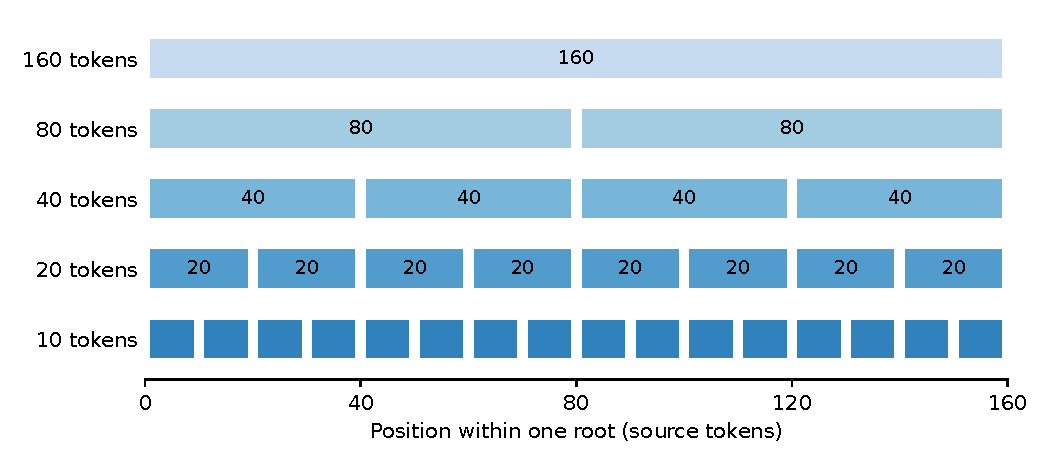
\includegraphics[width=\textwidth]{images/generated/tree_structure.pdf}
\caption{Aligned token spans within one complete 160-token root. Each
box is literal source text at a different scale. The illustration
shows containment, not measured relevance scores.}
\label{fig:tree}
\end{figure}

The level representation contains 85 features describing score
distributions separately at the five granularities. It includes summary
statistics, quantiles, concentration measures, softmax entropy, and
counts relative to score thresholds. The full tree representation adds
88 hierarchy-aware measurements for a total of 173. These include
parent--child gaps, sibling contrasts, and differences between adjacent
levels.

For example, a parent score minus the maximum child score describes
whether the coarse span matches the question better than its strongest
finer part. A mean child score measures a different property: whether
relevance is spread across the parent's descendants. Aggregating these
measurements across the paper gives a fixed-dimensional vector even
when papers have different numbers of chunks. The feature schema in
the repository defines the exact ordering and formulas.

The features use question-to-chunk similarity, not gold-evidence
similarity. Raw chunk embeddings are used to calculate scores but are
not concatenated as thousands of extra classifier inputs. A comparison
between stored/search scores and manually calculated cosine values
recorded a maximum absolute discrepancy of approximately
$1.09\times10^{-7}$, below the $10^{-5}$ audit tolerance.

\subsection{Linear and boosted-tree classifiers}
Phase 3A fits both level-only and full-tree linear classifiers. Five
paper-grouped training folds use seed 42. Nine candidates combine
learning rates 0.03, 0.01, and 0.003 with weight decays 0, 0.001, and
0.01. Each uses 300 full-batch epochs, training-fold standardisation,
and uniform cross-entropy. The hierarchy-based model is designated
the primary representation rather than chosen because of a favourable
validation result.

Phase 3B keeps those representations and replaces the linear classifier
with XGBoost. The grid combines maximum depths 2, 3, and 4; learning
rates 0.03 and 0.05; and 200 or 400 trees, giving 12 candidates per
representation. Other settings include minimum child weight 5,
row and column subsampling 0.8, L2 regularisation 1, and L1
regularisation 0. Square-root inverse-frequency weights address
class imbalance. Selection uses the grouped training folds, and the
tree model remains the primary method.

Simple score heuristics are also retained: maximum similarity,
top-five mean similarity, a training-tuned penalised top-five score,
and a leaf-breadth rule. Their purpose is to test whether broad
patterns are already captured by inexpensive hand-designed decisions.
Their reported classification results are not silently converted into
retrieval results where no corresponding evaluation was saved.

\section{Fusing language and similarity information}
\subsection{The initial fusion experiment}
Phase 3C combines a frozen Phase 2D classifier's five logits with the
173 tree features, producing 178 inputs to an XGBoost classifier.
An exploratory alternative concatenates its 1,024-dimensional hidden
representation with the same tree features, producing 1,197 inputs.
The primary logits-based variant is selected using training-fold
diagnostics.

There is an important weakness in this first procedure. The base Qwen
checkpoint has already been trained on all training questions. Its
features for those same questions are therefore in-sample features.
Dividing those rows into folds for the fusion classifier does not
undo that fact. The second-stage validation fold still contains
predictions produced by a base model that saw its labels during
training. The fusion cross-validation estimate is consequently
optimistic as an estimate of a fully unseen stacked pipeline.

The external validation predictions are not training rows for that
base fit, but the base checkpoint itself was selected using validation.
The original fusion result is retained as a development experiment
with these limitations, not presented as a clean final evaluation.

\subsection{Paper-grouped out-of-fold reconstruction}
Phase 3C-OOF reconstructs the language features correctly for the
meta-learner's training rows. For each of five paper-grouped folds,
Qwen is trained only on the other four folds and predicts the held-out
questions at a fixed third epoch. The fold sizes are 449, 449, 449,
450, and 448. Every training question receives a five-logit vector
from a model that did not train on that question's paper.

\begin{algorithm}[tbp]
\caption{Construction of out-of-fold language features}
\label{alg:oof}
\begin{algorithmic}[1]
\Require Training papers partitioned into folds $D_1,\ldots,D_5$
\For{$k=1,\ldots,5$}
  \State Train base router $f^{(-k)}$ on all papers outside $D_k$
  \State Use the fixed third-epoch checkpoint
  \For{question $q$ belonging to a paper in $D_k$}
    \State Store $\mathbf{z}^{\mathrm{OOF}}_q=f^{(-k)}(q)$
  \EndFor
\EndFor
\State Fit meta-model on $[\mathbf{z}^{\mathrm{OOF}}_q;\mathbf{x}^{\mathrm{tree}}_q]$
\State Refit the base router on all training papers for fixed three epochs
\State Predict validation logits with the refitted base router
\State Apply the meta-model to validation logits and tree features
\end{algorithmic}
\end{algorithm}

The full-data refit reproduces the fixed Phase 2D model state under the
recorded hash check. The fusion XGBoost configuration is inherited
and fixed at depth 2, learning rate 0.05, and 200 trees; this rerun does
not introduce another validation-tuned grid.

Out-of-fold construction fixes the in-sample base-feature problem.
It does not make every subsequent diagnostic fully nested: additional
meta-level cross-validation can still have dependencies through how
the base folds were constructed. Those diagnostics are not treated
as an unbiased nested estimate. Nor does this correction erase the
history of repeated external validation use.

\section{Expected-regret learning}
\label{sec:regret}
Phase 4 changes the question from \enquote{Which evidence-length class
is correct?} to \enquote{How much retrieval quality is lost by choosing
each size?} For every training question and size, define
\begin{equation}
C(q,g)=U^*(q)-U(q,g)\geq 0.
\label{eq:regret}
\end{equation}
Five XGBoost regressors predict these costs from the same 178-dimensional
combination of clean OOF Qwen logits and tree features. Each regressor
uses squared-error training, with the inherited fixed configuration
and no new hyperparameter search.

The routing rule is
\begin{equation}
\hat g(q)=\underset{g\in\granularities}{\arg\min}\,
\widehat C(q,g),
\label{eq:regretrule}
\end{equation}
with deterministic smaller-size tie-breaking. Since $U^*(q)$ is the
same for all candidate actions on a question, minimising true regret
is equivalent to maximising true retrieval utility. Under ideal
conditional-mean estimation, the same equivalence holds for expected
utility. In a finite fitted model, that reasoning motivates the
objective but does not guarantee that the selected action is optimal.

This formulation preserves information discarded by a single hard
label. Choosing a size whose F1 is almost maximal should incur a
small target cost even if it loses the argmax tie. Choosing a size
with much lower F1 should incur a larger cost. The regressors can
therefore learn useful distinctions between mistakes.

All 2,245 training utility vectors are complete in the final artifact.
Validation predictions are saved and hashed before the validation
utilities are read for scoring. Evaluation selects the corresponding
outcome from the five frozen actions rather than rerunning live
retrieval. This controls changes in the retrieval service and makes
the comparison an evaluation of the routing decision itself.

\section{Local tree-level routing}
\subsection{Changing the decision unit}
Phase 5A allows one paper to use several granularities for the same
question. The router is trained on the 4,081 gold-overlapping
question--tree pairs constructed in Chapter~\ref{ch:data}. Its
173-dimensional features have the same conceptual families as the
global tree representation but are computed within each local root.
The targets are local gold-overlap length categories.

The training class counts are $(557,876,1307,958,383)$ for the five
sizes. The XGBoost classifier inherits the fixed Phase 3B tree
configuration. Five paper-grouped folds provide diagnostics without
searching a new hyperparameter grid. No Qwen features are used in
this phase.

\subsection{Ranking trees and selecting chunks}
Trees are ranked independently of the predicted size. The score of
tree $T$ is an equal-weight average of its level-wise mean similarities:
\begin{equation}
S(q,T)=\frac{1}{|\granularities|}
\sum_{g\in\granularities}
\frac{1}{|\mathcal{C}_g(T)|}
\sum_{c\in\mathcal{C}_g(T)}s(q,c),
\label{eq:treescore}
\end{equation}
using available descendants and the implementation's handling of
partial edge trees. Equal weighting of levels prevents the sixteen
10-token leaves from dominating solely because they are more numerous.
It does not prove that the score is an optimal relevance estimator.

The five highest-ranked roots are retained. Within each root, the
classifier predicts a size and the single most similar chunk at that
size is returned. The primary output therefore contains five chunks,
potentially of different lengths. The router does not inspect gold
overlap to select validation trees.

The matched baseline uses exactly the same tree ranking, top-five
roots, and one-chunk-per-tree rule, but fixes the size to 40.
Additional fixed sizes are evaluated in the same way. This comparison
isolates the local size decision more directly than comparison with
global fixed-40 retrieval, which can select several chunks from one
root.

An exploratory variant returns all descendants at the predicted level
within each selected root. That variant changes the output budget
and is reported separately. Its additional evidence coverage cannot
be credited to a better five-chunk decision.

\section{A frozen context-need feature}
\subsection{Free generation and the validity gate}
Phase 5B asks whether a cheap semantic summary of the question can
help the local router. The frozen post-trained Qwen model predicts
one of three context-need categories: short, medium, or long. The
category is one-hot encoded and appended to each local tree feature
vector for that question, increasing the dimension from 173 to 176.
The language model is not fine-tuned on the local labels.

The first version uses deterministic free generation with a limit of
eight new tokens. It produces invalid responses on part of both splits,
including answers to the question instead of a category. The pipeline's
gate forbids replacing those failures with an arbitrary default and
proceeding as if the input feature were valid. No downstream classifier
result is claimed for that version.

\subsection{Constrained first-token scoring}
The repaired version first tests revised wording on the 175 previously
invalid training questions. It then uses a stronger output contract:
compare only the next-token logits for the verified single tokens
\texttt{short}, \texttt{medium}, and \texttt{long}, whose IDs are 8412,
25252, and 4670. One forward pass and an argmax produce a category;
there is no free text to parse.

The revised prompt explicitly tells the model not to answer the
question and to provide one lowercase label only. The full wording
is recorded in Appendix~\ref{app:protocols}. The training-only prompt
probe and final constrained evaluation are different operations:
the former tests wording on known training failures, while the latter
enforces validity for all required feature rows.

The local training examples, labels, tree ranking, and boosted-tree
protocol remain unchanged. The language model is frozen and receives
no task-label updates, so an OOF fine-tuning procedure is not required
to remove supervised in-sample predictions from this particular
feature. The experiment still shares the broader development-set
limitations of the rest of the thesis.

\section{What is held constant, and what is not}
Some comparisons isolate one change, such as the Phase 2C/2D prompt
or the Phase 5A/5B-v2 feature addition. Others redesign several
components, including the move from numeric generation to aliases
and from global to local routing. The results therefore distinguish
controlled effects from descriptive cross-phase differences.
